\documentclass[journal]{IEEEtran}
\usepackage{amsmath,amssymb,amsthm}
\usepackage{graphicx}
\usepackage{booktabs}
\usepackage{url}
\usepackage[hidelinks]{hyperref}
\usepackage{cite}
\newtheorem{proposition}{Proposition}
\newtheorem{corollary}{Corollary}
\newcommand{\BA}{\mathrm{BA}}

\begin{document}
\title{How Many Unlabeled Observations Does Subject Centering Need? A Reference-Size Law for Cross-Participant EEG Decoding}
% Author order follows the earlier letter. Affiliations, contact address, and order await author approval.
\author{Andrew~A.~Lane, Brady~D.~Nelson, and~Wendy~Tang}
\markboth{Draft, 22 November 2026}{Lane \MakeLowercase{\textit{et al.}}: A Reference-Size Law for Subject Centering}
\maketitle

\begin{abstract}
Subtracting each participant's mean feature vector is a simple remedy for the between-participant variability that dominates cross-participant EEG decoding. We treat the step as an estimate of a participant offset from $m$ unlabeled reference observations and derive its consequences. The squared separation of two conditions after centering is $m/(m+1)$ times its asymptote, centering helps only above a break-even reference size $m^\ast$ fixed by the share of discriminant variance that belongs to participants, and in a complete repeated-measures panel leave-one-out centering is an exact rescaling of full-panel centering. On single trials of five public ERP CORE paradigms the law predicts accuracy at six reference sizes with a mean absolute error of 0.004, and the predicted break-even size agrees with the observed one in all five. Single-trial gains are small, from 0.000 to 0.036 balanced accuracy. On trial-averaged affective ERPs of 211 participants, where the participant share is large, centering on a three-condition panel raises three-class accuracy from 0.679 to 0.900, a two-condition panel gives 0.820, and a single observation gives none of the gain. Euclidean alignment recovers 0.834 on averages and nothing on single trials, which separates a participant gain from a participant offset. The results specify when subject centering is a valid description of deployment: the test participant must supply unlabeled reference observations, and their number sets the gain.
\end{abstract}

\begin{IEEEkeywords}
EEG decoding, cross-subject generalization, subject centering, transductive normalization, Euclidean alignment, event-related potentials, repeated measures.
\end{IEEEkeywords}

\section{Introduction}
\IEEEPARstart{B}{etween-participant} variability is the main obstacle to EEG decoders that generalize to people absent from training \cite{saha2020variability,wu2022transfer}. In affective ERP data the participant factor carries several times the variance of the experimental condition. A family of label-free alignment methods addresses this by transforming each participant's data with statistics of that participant alone. Euclidean alignment whitens each participant's trials by their mean spatial covariance \cite{he2020ea}, and Riemannian methods recenter covariance matrices on the manifold \cite{zanini2018transfer,rodrigues2019rpa}. Subject centering is the first-order member of the family. It subtracts the participant's mean feature vector, and in repeated-measures ERP designs it produces large accuracy gains.

All of these methods are transductive. They use unlabeled observations of the test participant, and a reported gain describes deployment only if those observations exist when the decoder is applied. Three questions decide what a centering gain means, and the literature leaves them open. How many reference observations does the estimate need? When does centering lower accuracy? And what does a complete within-participant panel contribute beyond the offset estimate, given that its composition is fixed by the experimental design?

This paper answers them with a single additive model. The contributions are a reference-size law for the separation after centering (Proposition~\ref{prop:law}), a break-even reference size below which centering lowers accuracy (Corollary~\ref{cor:breakeven}), exact identities for the complete balanced panel, including the equivalence of leave-one-out and full-panel centering (Proposition~\ref{prop:panel}), and tests of each prediction on five public ERP CORE paradigms \cite{kappenman2021erpcore} and on trial-averaged affective ERPs of 211 participants, with Euclidean and Riemannian alignment evaluated on the same reference sets. The work is the geometric-transparency level of the ARSPI-Net framework \cite{lane2026dissertation,lane2026bibm} stated as a general result about EEG features.

\section{Theory}\label{sec:theory}

\subsection{Observation Model}
Participant $s$ contributes observations $\mathbf{x}_{s,i}\in\mathbb{R}^d$ with labels $c_{s,i}\in\{1,\dots,K\}$,
\begin{equation}
\mathbf{x}_{s,i}=\mathbf{a}_s+\boldsymbol\mu_{c_{s,i}}+\mathbf{e}_{s,i}, \label{eq:model}
\end{equation}
where $\mathbf{a}_s$ is a participant offset with covariance $\Sigma_a$, $\boldsymbol\mu_c$ is the condition mean, and $\mathbf{e}_{s,i}$ is zero-mean noise with covariance $\Sigma_e$, independent across observations and of $\mathbf{a}_s$. An observation is a trial in single-trial decoding and a condition average in ERP decoding. For a pair of conditions with $\Delta\boldsymbol\mu=\boldsymbol\mu_c-\boldsymbol\mu_{c'}$, the squared Mahalanobis separation of an uncentered observation across participants is
\begin{equation}
D_0^2=\Delta\boldsymbol\mu^\top(\Sigma_a+\Sigma_e)^{-1}\Delta\boldsymbol\mu. \label{eq:d0}
\end{equation}

\subsection{Reference Centering}
Let $\mathcal{R}_s$ be a set of $m$ unlabeled reference observations of participant $s$ with class proportions $\boldsymbol\pi_s$, and let $\bar{\mathbf{x}}_{\mathcal{R}_s}$ be their mean. Reference centering forms $\tilde{\mathbf{x}}_{s,i}=\mathbf{x}_{s,i}-\bar{\mathbf{x}}_{\mathcal{R}_s}$.

\begin{proposition}[Reference-size law]\label{prop:law}
Let observation $i\notin\mathcal{R}_s$. Under \eqref{eq:model},
\begin{equation}
\tilde{\mathbf{x}}_{s,i}=\boldsymbol\mu_{c_{s,i}}-\textstyle\sum_c\pi_{s,c}\boldsymbol\mu_c+\mathbf{e}_{s,i}-\bar{\mathbf{e}}_{\mathcal{R}_s}, \label{eq:centered}
\end{equation}
which contains no participant offset and has noise covariance $(1+1/m)\Sigma_e$. If $\boldsymbol\pi_s=\boldsymbol\pi$ for all participants, the separation of two conditions is
\begin{equation}
D^2(m)=\frac{m}{m+1}\,D_\infty^2,\qquad D_\infty^2=\Delta\boldsymbol\mu^\top\Sigma_e^{-1}\Delta\boldsymbol\mu. \label{eq:law}
\end{equation}
\end{proposition}
\begin{proof}
Average \eqref{eq:model} over $\mathcal{R}_s$ and subtract. The offset $\mathbf{a}_s$ cancels exactly. The two noise terms are independent because $i\notin\mathcal{R}_s$, which gives the covariance. With a common $\boldsymbol\pi$ the subtracted mean term is the same constant for every participant and condition, so it leaves $\Delta\boldsymbol\mu$ unchanged.
\end{proof}

\begin{corollary}[Break-even reference size]\label{cor:breakeven}
Let $r=D_0^2/D_\infty^2\in(0,1]$. Reference centering improves on the uncentered readout if and only if
\begin{equation}
m>m^\ast=\frac{r}{1-r}. \label{eq:breakeven}
\end{equation}
\end{corollary}
\begin{proof}
$D^2(m)>D_0^2$ is $m/(m+1)>r$.
\end{proof}

The ratio $r$ is the share of discriminant-direction variance that is not participant variance. When observations are averages of $k$ trials, $\Sigma_e$ is replaced by $\Sigma_e/k$ while $\Sigma_a$ is unchanged, so $r$ falls toward zero as $k$ grows and $m^\ast$ falls with it. Averaged ERPs are therefore the regime where one or two reference observations already give a large gain, and single trials are the regime where $r$ is close to one, the gain is small, and a reference set below $m^\ast$ lowers accuracy. When the reference observations are drawn without regard to class, the reference mean also carries the between-class spread $\Sigma_\mu$, and $\Sigma_e/m$ in the reference term becomes $(\Sigma_e+\Sigma_\mu)/m$, a small correction when single-observation effects are weak.

Three further consequences follow. First, the gain over \eqref{eq:d0} is set by how much participant variance lies along the discriminant, $D_\infty^2/D_0^2\ge1$, and it saturates quickly in $m$: one reference observation recovers half of $D_\infty^2$ and ten recover $91\%$. Second, when $\boldsymbol\pi_s$ varies across participants, the term $\sum_c\pi_{s,c}\boldsymbol\mu_c$ becomes a participant-specific shift along the condition means, and centering reintroduces a participant effect that is correlated with class composition. Designs with fixed condition proportions are free of it. Third, \eqref{eq:law} needs no label from the test participant, but it does need $m\ge1$ further observations of that participant. With $m=0$ the transform is undefined, and the decoder falls back to \eqref{eq:d0}.

\subsection{The Complete Balanced Panel}
In a repeated-measures design every participant contributes each condition once, so $K$ observations form a panel with $\boldsymbol\pi=\mathbf{1}/K$. Full-panel centering subtracts the mean of all $K$ observations, including the one being classified.

\begin{proposition}[Panel identities]\label{prop:panel}
For a complete balanced panel, (i) $\tilde{\mathbf{x}}_{s,c}=\boldsymbol\mu_c-\bar{\boldsymbol\mu}+\mathbf{e}_{s,c}-\bar{\mathbf{e}}_s$, with noise covariance $(1-1/K)\Sigma_e$ and cross-covariance $-\Sigma_e/K$ between two observations of the same panel. (ii) Leave-one-out centering satisfies
\begin{equation}
\mathbf{x}_{s,c}-\frac{1}{K-1}\sum_{c'\ne c}\mathbf{x}_{s,c'}=\frac{K}{K-1}\,\tilde{\mathbf{x}}_{s,c}. \label{eq:loo}
\end{equation}
(iii) Both forms give $D^2=\frac{K}{K-1}D_\infty^2$ for a single observation of the panel.
\end{proposition}
\begin{proof}
(i) follows from \eqref{eq:model}. For (ii), $\sum_{c'\ne c}\mathbf{x}_{s,c'}=K\bar{\mathbf{x}}_s-\mathbf{x}_{s,c}$, and collecting terms gives the factor $K/(K-1)$. (iii) follows from (i), and from Proposition~\ref{prop:law} with $m=K-1$ after noting that the leave-one-out reference set contains every condition except $c$, which scales $\Delta\boldsymbol\mu$ by $K/(K-1)$.
\end{proof}

Identity \eqref{eq:loo} shows that leave-one-out centering is a rescaling of full-panel centering. It carries the same information for any scale-equivariant readout, so it is a consistency check of the implementation and not an independent control. The separation in (iii) exceeds $D_\infty^2$ because the reference set of a panel is label-structured: it is known to contain the other conditions and not the one being classified. The panel therefore supplies design knowledge in addition to the offset estimate. The readout that uses all of it assigns the $K$ labels of a test panel jointly, as the permutation $\sigma$ maximizing $\sum_c\log p(\sigma(c)\mid\tilde{\mathbf{x}}_{s,c})$, and the negative cross-covariance in (i) is what a joint assignment exploits.

\subsection{Incomplete Panels and Second-Order Alignment}
If a test participant contributes a subset $\mathcal{A}$ of the conditions, centering still removes $\mathbf{a}_s$, and the class means become $\boldsymbol\mu_c-\bar{\boldsymbol\mu}_\mathcal{A}$. A readout trained on complete panels then meets a shift $\bar{\boldsymbol\mu}-\bar{\boldsymbol\mu}_\mathcal{A}$ that depends on which conditions are present, and its accuracy falls between the complete-panel and uncentered values.

Euclidean alignment \cite{he2020ea} and Riemannian recentering \cite{zanini2018transfer} use the same unlabeled reference set to whiten each participant's second-order statistics. Under the purely additive model \eqref{eq:model} they leave $\mathbf{a}_s$ in place. They remove it only to the extent that the participant effect is multiplicative, $\mathbf{x}_{s,i}=g_s(\boldsymbol\mu_c+\mathbf{e}_{s,i})$ with a participant gain $g_s$, because whitening by the participant's own second moment divides out $g_s$. Comparing the two families on the same panels therefore measures how much of the participant effect is an offset and how much is a gain.

\section{Materials and Methods}
\subsection{Datasets}
\emph{ERP CORE} \cite{kappenman2021erpcore}: five stimulus-locked paradigms (N170, P3, N400, N2pc, MMN) with 40 participants each, delivered as ICA-corrected, baseline-corrected epochs at 256~Hz with 28 scalp channels. Trials flagged by the provided artifact detection are removed. \emph{SHAPE}: trial-averaged ERPs from passive viewing of negative, neutral, and pleasant pictures, 34 channels, one average per participant and condition. One participant with an all-zero epoch is excluded, leaving 211 participants and 633 observations. All inputs are unscaled microvolts, so no per-epoch statistic enters the features.

\subsection{Single-Trial Experiment}
Features are post-stimulus means in 31~ms bins for each channel. Decoding is across participants with five participant-grouped folds, feature standardization and a class-balanced L2 logistic readout ($C=0.1$) fitted on training participants. Participants with fewer than 64 retained trials or fewer than five trials in a class are not used. Training participants are centered on the mean of all their trials. For a test participant the reference mean is taken over all trials, over $m\in\{1,2,4,8,16,32\}$ trials drawn at random without regard to class and removed from the test set (five draws), or over the preceding trials in recorded order (a causal running mean). Euclidean alignment uses the participant's mean spatial covariance over all trials. The prediction for each $m$ is $\Phi\big(\Phi^{-1}(\BA_\infty)\sqrt{m/(m+1)}\big)$ with $\BA_\infty$ the all-trial accuracy, and the predicted break-even size uses \eqref{eq:breakeven} with $r=\big(\Phi^{-1}(\BA_0)/\Phi^{-1}(\BA_\infty)\big)^2$. The law and its probit form were written into the experiment file before the run.

\subsection{Panel Experiments}
On SHAPE each epoch is flattened and decoded with participant-grouped 10-fold cross-validation, standardization, and an L2 logistic readout ($C=0.1$). Test-side rules are the full three-condition panel, leave-one-out centering, a panel of two randomly chosen conditions (five draws), and a single observation. The alignment comparison applies each transform of Table~\ref{tab:shape} to training and test participants alike, using only each participant's own panel. Tangent-space features use log-Euclidean maps of ridge-regularized spatial covariances. The joint-assignment readout gives each test panel the label permutation with the largest total log-probability. On ERP CORE, participant-condition averages form complete two-condition panels, decoded with participant-grouped five-fold cross-validation repeated five times. Intervals are percentile bootstraps over participants, and nulls permute labels within participants.

\section{Results}\label{sec:results}
\subsection{The Reference-Size Law on Single Trials}
Fig.~\ref{fig:law} shows cross-participant single-trial accuracy as a function of the reference size. In every paradigm accuracy rises with $m$ along the curve of Proposition~\ref{prop:law}. Over the 30 points (five paradigms, six sizes) the mean absolute difference between observed and predicted balanced accuracy is 0.004 and the largest is 0.017, at $m=1$ in N170. The prediction uses the all-trial accuracy of each paradigm, so agreement at $m=32$ is close by construction, and the informative comparison is at small $m$: for $m\ge2$ the mean absolute difference is 0.003. At $m=1$ the observed value is below the prediction in four paradigms, the direction expected from the between-class term $\Sigma_\mu/m$ of a reference drawn without regard to class.

\begin{figure*}[t]
\centering
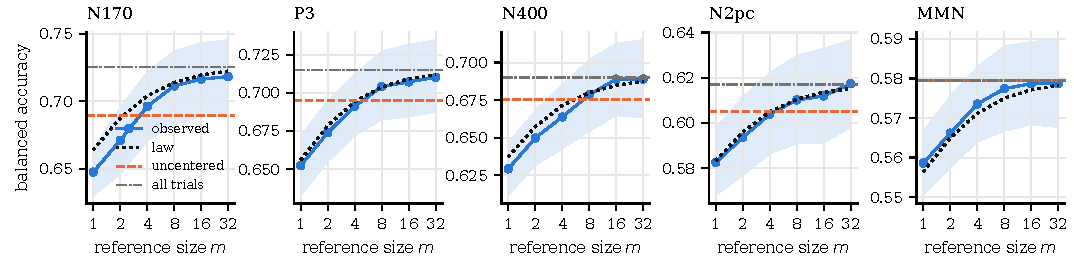
\includegraphics[width=\textwidth]{figures/fig_law.pdf}
\caption{Reference-size law on single trials of ERP CORE, cross-participant decoding, chance 0.5. Observed balanced accuracy with participant-bootstrap 95\% intervals against the prediction $\Phi(\Phi^{-1}(\BA_\infty)\sqrt{m/(m+1)})$, which uses the all-trial accuracy alone. Dashed: uncentered readout. Mean absolute error over the 30 points is 0.004.}
\label{fig:law}
\end{figure*}

Table~\ref{tab:erpcore} gives the end points. Centering on all trials of the test participant raises accuracy by 0.036 [0.021, 0.052] for N170, 0.020 for P3, 0.015 for N400, and 0.012 for N2pc, and leaves MMN unchanged ($-0.000$ [$-0.002$, $+0.002$]). The causal running mean reaches 0.721, 0.710, 0.684, 0.616, and 0.580, within 0.006 of the all-trial value in every paradigm, so the transform has an online form. Below the break-even size centering lowers accuracy: with one reference trial N170 falls from 0.690 to 0.648. Corollary~\ref{cor:breakeven} predicts the crossing from the two end points alone, at $m^\ast=2.2$, 4.2, 5.2, and 4.0, and never for MMN, where the participant share is zero. On the tested grid the first size above the uncentered readout is 4, 8, 8, and 8, and none for MMN, each the smallest grid value above its $m^\ast$. For N2pc, whose predicted break-even size is 4.0, accuracy at $m=4$ equals the uncentered value to three decimals (0.604 against 0.605).

\begin{table*}[t]
\centering
\caption{ERP CORE. Left: participant-condition averages, complete two-condition panels (chance 0.5). Right: cross-participant single-trial decoding with the participant mean taken over all trials, the gain over the uncentered readout with participant-bootstrap 95\% interval, the gain of Euclidean alignment, the break-even reference size $m^\ast$ predicted by \eqref{eq:breakeven}, and the smallest tested $m\in\{1,2,4,8,16,32\}$ whose accuracy exceeds the uncentered readout.}
\label{tab:erpcore}
\begin{tabular}{lcc|cccccc}
\toprule
 & \multicolumn{2}{c|}{Averages} & \multicolumn{6}{c}{Single trials} \\
Paradigm & Uncentered & Panel centered & Uncentered & Centered & Centering gain & Alignment gain & $m^\ast$ & First $m$ above \\
\midrule
N170 & 0.735 & 0.965 & 0.690 & 0.725 & $+0.036$ [$+0.021$, $+0.052$] & $+0.004$ [$-0.011$, $+0.020$] & 2.2 & 4 \\
P3 & 0.832 & 0.995 & 0.695 & 0.715 & $+0.020$ [$+0.007$, $+0.031$] & $-0.003$ [$-0.019$, $+0.012$] & 4.2 & 8 \\
N400 & 0.868 & 1.000 & 0.675 & 0.690 & $+0.015$ [$+0.003$, $+0.027$] & $-0.008$ [$-0.021$, $+0.005$] & 5.2 & 8 \\
N2pc & 0.636 & 0.867 & 0.605 & 0.617 & $+0.012$ [$+0.006$, $+0.018$] & $+0.010$ [$-0.001$, $+0.020$] & 4.0 & 8 \\
MMN & 0.872 & 0.955 & 0.580 & 0.579 & $-0.000$ [$-0.002$, $+0.002$] & $+0.005$ [$-0.000$, $+0.011$] & $\infty$ & none \\
\bottomrule
\end{tabular}
\end{table*}


\subsection{Complete Panels}
With participant-condition averages the participant share is large and the panel is complete. On ERP CORE, panel centering raises two-class accuracy in all five paradigms (Table~\ref{tab:erpcore}), for example from 0.735 to 0.965 for N170 and from 0.636 to 0.867 for N2pc, each above its within-participant permutation null ($p=0.002$, the floor of 500 permutations). On SHAPE, with three conditions and 211 participants, the uncentered readout scores 0.679 and full-panel centering 0.900, a gain of $+0.221$ [$+0.188$, $+0.256$], against a within-participant permutation null with mean 0.335 and maximum 0.403 over 100 permutations. Leave-one-out centering scores 0.904, as \eqref{eq:loo} requires of a rescaled copy of the same features. A panel of two of the three conditions gives 0.820, and a single observation, for which no reference exists, is decoded by the uncentered readout at 0.679. A readout trained on centered panels and applied to an uncentered single observation scores 0.509. The gain persists when the input is scaled by per-epoch z-scoring or by its pre-stimulus standard deviation ($+0.203$ and $+0.219$ on the 212-participant cohort of the original analysis), so it is not produced by per-epoch scaling. In the flattened epoch the participant factor carries 70.6\% of the variance, the condition factor 8.8\%, and the residual 20.6\%.

\begin{table}[t]
\centering
\caption{SHAPE, three affective conditions (chance 0.333), 211 participants, unscaled epochs, participant-grouped 10-fold cross-validation. Balanced accuracy with participant-bootstrap 95\% intervals. Every transform uses only the participant's own unlabeled panel.}
\label{tab:shape}
\begin{tabular}{llc}
\toprule
Transform & Order & Balanced accuracy \\
\midrule
None & -- & 0.679 [0.646, 0.712] \\
Euclidean alignment & second & 0.834 [0.806, 0.863] \\
Tangent space, cohort reference & -- & 0.472 [0.439, 0.507] \\
Tangent space, participant recentering & second & 0.727 [0.690, 0.765] \\
Panel centering & first & 0.900 [0.872, 0.927] \\
Panel centering and scaling & first & 0.905 [0.875, 0.932] \\
Euclidean alignment, then centering & both & 0.912 [0.883, 0.937] \\
Panel centering, joint assignment & first & 0.953 [0.926, 0.976] \\
\bottomrule
\end{tabular}
\end{table}


\subsection{Alignment Alternatives and Joint Assignment}
Table~\ref{tab:shape} compares transforms that use the same unlabeled panel. Euclidean alignment reaches 0.834, a gain of $+0.155$ [$+0.120$, $+0.190$] over the uncentered readout. The prediction written before the run, that a second-order transform would stay near the uncentered readout as the additive model implies, was not borne out on these averages, and it held on single trials (Table~\ref{tab:erpcore}). Centering exceeds alignment by $+0.066$ [$+0.036$, $+0.096$], and alignment followed by centering scores 0.912, a difference of $+0.011$ [$-0.017$, $+0.038$] from centering alone. Adding a per-feature scale from the three-observation panel changes centering by $+0.005$ [$-0.016$, $+0.027$]. In the covariance domain, tangent-space features with a cohort reference score 0.472 and participant recentering raises them to 0.727 ($+0.253$ [$+0.209$, $+0.299$]). These features discard the time course of the average, which accounts for their lower level. Joint assignment of the three labels of each test panel raises the centered readout from 0.900 to 0.953, a gain of $+0.052$ [$+0.028$, $+0.076$] that comes entirely from the known composition of the panel.

\section{Discussion}
\subsection{What a Centering Gain Measures}
The additive model accounts for the observations across two datasets, two regimes, and eight transforms. Centering is an estimate of a participant offset, its benefit is set by the participant share of discriminant variance, and its cost is the noise of the estimate, $\Sigma_e/m$. Single trials sit where the share is small. There the full gain is between 0.000 and 0.036, a reference set of one or two trials lowers accuracy, and the break-even size of Corollary~\ref{cor:breakeven} locates the crossing in all five paradigms from two numbers, the uncentered and the fully centered accuracy. Trial-averaged ERPs sit where the share is large, because averaging divides $\Sigma_e$ by the number of trials and leaves $\Sigma_a$ unchanged. There a panel of two reference observations already carries most of the gain.

\subsection{Offsets and Gains}
Second-order alignment and first-order centering act on different parts of the participant effect. On single trials Euclidean alignment changes accuracy by 0.010 or less in every paradigm, with intervals that include zero, while centering gives a positive gain in four of five. On trial-averaged ERPs alignment alone recovers about 70\% of the centering gain, which the additive model does not predict. A participant gain, a multiplicative scale on the whole response, is therefore a substantial part of between-participant variability in averaged ERPs. Centering removes the offset and leaves a gain in place, alignment divides out the gain and leaves the offset, and on these data the offset is the larger part ($+0.066$ [$+0.036$, $+0.096$] for centering over alignment). The two families are complementary in the model, and on averaged data their combination adds no measurable accuracy over centering alone.

\subsection{Reporting Transductive Results}
A decoding accuracy obtained with any participant-level transform should state three things: which observations of the test participant the transform used, whether they include the observation being classified, and whether their class composition was fixed by the design. With a complete balanced panel, cross-participant classification becomes a within-participant contrast with separation $K/(K-1)$ times the asymptote, and the joint-assignment readout raises accuracy further by using the known composition. Such a result describes a repeated-measures protocol in which every test participant is recorded in every condition. It is a different quantity from the accuracy of a decoder applied to one new observation of a new participant, and the two belong in separate columns of any comparison.

\subsection{Scope and Future Directions}
The present work characterizes linear readouts of time-domain ERP features in six paradigms. The law is stated for a common class composition across participants, and Proposition~\ref{prop:law} predicts a participant-specific shift when the composition varies, which the oddball paradigms with resampled class proportions can measure directly. Extending the reference-size analysis to covariance-domain alignment, where the reference estimate is a matrix and its error grows with the channel count, would give Euclidean and Riemannian alignment their own break-even sizes. Motor-imagery and steady-state paradigms, with oscillatory features, are a natural next test of how the participant share $r$ varies across signal types.


\section*{Ethics, Data, and Code Availability}
The SHAPE study was collected by the Stony Brook University Laboratory for Clinical Affective Neuroscience under that laboratory's Institutional Review Board oversight. ERP CORE is a publicly released dataset governed by its original collection protocol \cite{kappenman2021erpcore}.
SHAPE data are available from the Laboratory for Clinical Affective Neuroscience at Stony Brook University on request. Analysis code and aggregate results are available from the corresponding author on request.

\section*{Use of AI-Assisted Tools}
An AI assistant (Claude, Anthropic) was used to write analysis code, run experiments, search the literature, and draft text under the direction of the authors. The authors reviewed every analysis and statement, and take full responsibility for the content.

\bibliographystyle{IEEEtran}
\bibliography{refs}
\end{document}
